%-----------------------------------------------------------%

The generation of simulated images involves several steps. These are summarised in the following block-level flowchart -

\begin{Flowchart}[h!]
    \centering
    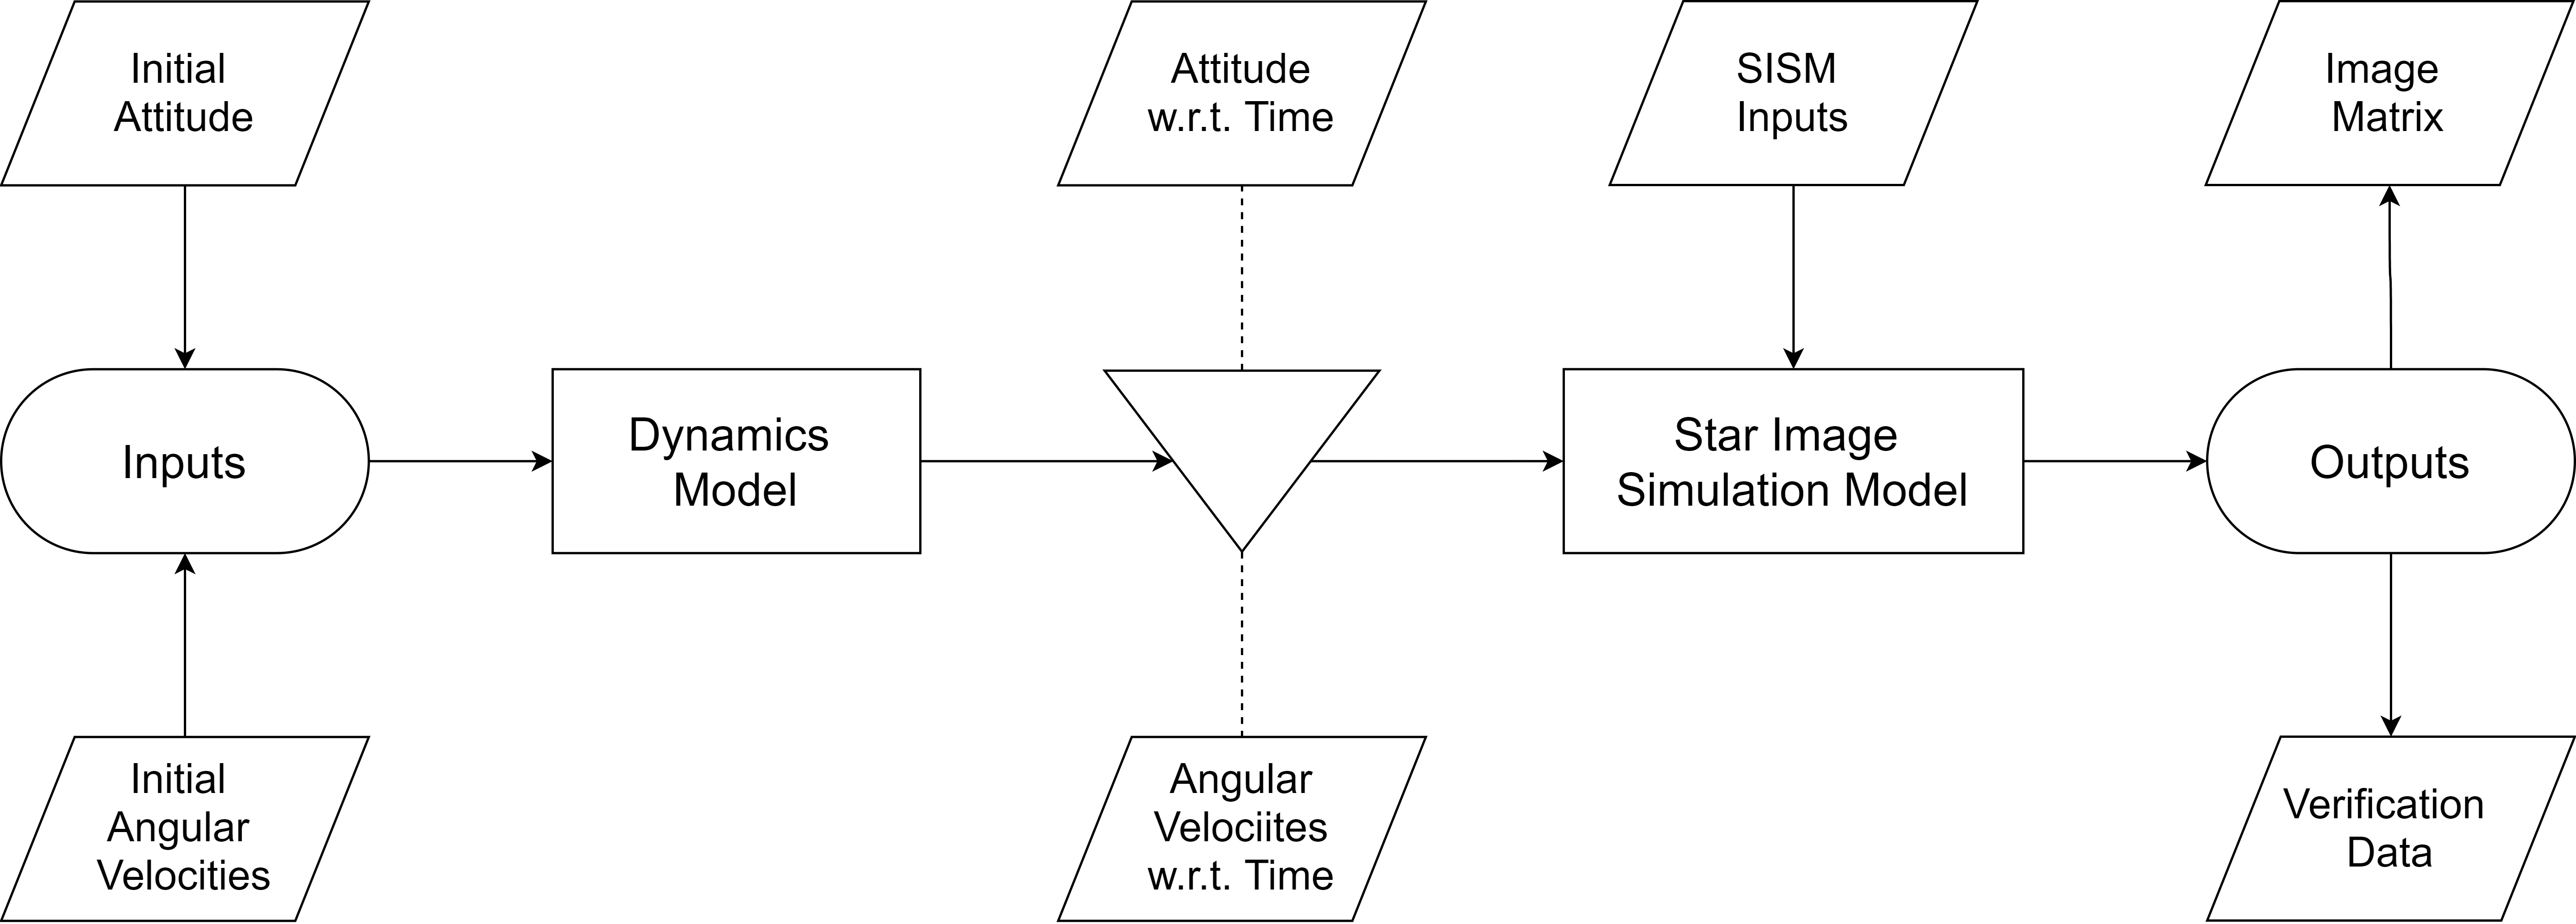
\includegraphics[scale=0.06]{Figures/Model/se_BLock_Level_Diagram.png}
    \caption{Star Image Simulation Block Level}
    \label{fig:SIS_Block}
\end{Flowchart}

% Block wise Flowchart

% \subsubsection{Inputs}
% \blindtext
% % Star Catalogue
% % Global Inputs
% % Boresight Inputs - Attitude + Angular Velocities
% % Lens Inputs
% % Sensor Inputs
% % Image Generation Inputs? 
% % Noise Inputs 

% \subsubsection{Pre-processing} % 2 parts - Loading constants, and Pre-processing of Catalogue
% \blindtext

% \subsubsection{Light Model}
% \blindtext

% \subsubsection{Lens Model} % Seidel Coefficients, Simplistic Model
% \blindtext

% \subsubsection{CMOS Model} % What happens in the Sensor
% Visual information is recorded via the CMOS sensor placed at the focal plane of the optics system to measure the light gathered during the exposure. The sensor is platted into an array of pixels, each of which is tasked to gather the light arriving within a small patch of sensor area. The efficiency with which the sensor and its pixels gather light, and the accuracy to which it determines the amount gathered by each pixel, are crucial in determining the quality of the recorded image. \cite{DSLRs} 

% Hence, we need to have an accurate model for the CMOS Sensor. The noise effects in the CMOS Sensor have been separated out into the Noise Model; thus, this CMOS Model takes the input as the wavefront incident on the sensor due to the stars, and produces a no-noise matrix of pixel values as seen by the sensor. 

% \subsubsection{Noise Model} % Introduction to noise model
% The incoming light from the stars is the signal we need the CMOS Imaging Sensor to transcribe faithfully; inaccuracies in the recording process constitute noise, and inhibit the ability to reconstruct the Star Vectors in the image frame, which leads to inaccuracies in the Star Tracking and Star Matching Algorithms. In order to extract the best performance from the CMOS Imaging Sensor, it is helpful to have an understanding of the various contributions to image noise and how various design choices in the Lens System and the choice of CMOS Sensor affect this noise.


% \subsubsection{Slew Model} % Sum images over different time instants
% \blindtext

% % ---------------------- %
% % Noise Model - Detailed %
% % ---------------------- %



% \subsection{Noise Model}
% There are several image sensor noise sources that must be simulated in the camera model. Our image sensor of choice is a CMOS sensor, and so, we have focused on the noises specific to a CMOS Sensor. The noises that have been considered in the Sensor Model, in a chronological order are - \emph{Background Light, Photon Shot Noise, Quantum Efficiency, Parasitic Light Sensitivity, Photo-Response Non-Uniformity, Fixed Pattern Noise, Dark Noise, Pixel Storage Node Leakage, Dead Pixels} and \emph{Read Noise}.

% The order is based on the following information - 
% The background light is due to the ambient light level throughout the universe. This is a constant value and this needs to be added first. Next, the photons have dual nature, due to which, their detection at the CMOS Sensor follows Poisson Distribution, captured by the Photon Shot Noise. Both of these noises / errors are from before the photons even strike the Sensor.

% Next, as the photons strike the photodiodes, not all the photons are converted to photoelectrons. This is captured by the Quantum Efficiency. 

% Now, we have 2 noises that are dependent on the inputs - Parasitic Light Sensitivity, and the 


% \subsubsection{Background Light} % 2.
% Background Light/noise, or ambient noise, is the noise introduced in the image which can come from various uncontrollable sources,like other celestial sources or cosmic radiation. The photoelectron density that is formed in the process of background imaging can be expressed as follows:
% \begin{equation}
%   b=\int{b_oA\tau(\lambda)P(\lambda)A_pt_s} d\lambda
% \end{equation}
% Where, b0 = 5 x 10$^(10) = 2.512^Mb$ , 
% Mb stands for the magnitude order of the background which can be generally of brightness of 10.0 Mv. 
% \\A$_p$ stands for Area of a Single Pixel,
% \\A stands for Optical Entrance Pupil Area,
% \\$\tau (\lambda)$ is the Optical Transmittance,
% \\P($\lambda$) is the Spectral Response, and
% \\t$_s$ is the Integration Time.


% \subsubsection{Photon Shot Noise} % 3.
% Image sensors measure scene irradiance by counting the number of discrete photons incident on the sensor over a given time interval. The independence of random individual photon arrivals leads to photon noise, a signal dependent form of uncertainty that is a property of the underlying signal itself. Individual photon detections can be treated as independent events that follow a random temporal distribution. As a result, photon counting is a classic Poisson process.Even from Quantum Statistics, when collecting photons from an unvarying source over a set amount of time, we get a Poisson Distribution.Hence, If the mean value of the number of photons that hit the sensor is n, the RMS noise(variance in the number of photons) is the square root of n.

% The formula used in the code is:

% Pixel Value = poissrnd(Pixel Value)




% \subsubsection{Quantum Efficiency} % 1. Quantum Efficiency% 
% Quantum efficiency (QE) is one of the most important characteristics of any electro-optical
% device including the CMOS image sensor. QE is the ratio of average number of electrons
% generated in the pixel ($\mu$e) to the average number of impinging photons ($\mu$p) 
% on the pixel during exposure time.When talking about sensitivity, QE plays an important role, as well as
% the pixel sensitive area and the use of microlenses. QE can also be defined as the 
% measure of how efficiently the sensor converts light (photons) to charge
% (electrons). The more electrons in a pixel during the integration period, the
% higher the output level of the sensor, so the more sensitive the sensor is for
% that specific wavelength of the light. A QE of 1 means that every photon
% generates (in average) one electron. Normally the QE is less than 1 (or 100%).
% Read noise and QE combined gives the overall sensitivity of the sensor as QE/Read
% Noise, or the minimum amount of light you can see.
% Formula used to calculate this:
% \begin{equation}
%     QE(\lambda)= \mu_e/\mu_p
% \end{equation}



% \subsubsection{Parasitic Light Sensitivity} % ???
% Parasitic Light Sensitivity (PLS) is the ratio of the light sensitivity of the photodiode to the light sensitivity of the Memory Node (also called the Storage Node) in Global Shutter. \newline

% Parasitic Light Sensitivity Noise (PLSN) is due to the light incident into Memory Node. An increase of PLS leads to a deterioration in the image quality.  This  is  because  the  photo-electrons  generated  by  incident  light  to  Memory Node  are  added  to  the  photo-electrons stored in Memory Node after the exposure. \newline

% The Memory Node is about 80,000x more sensitive than the Photodiode. However, the Memory Node is susceptible to photons only after the Shutter Closes. So, the time to be taken into account is $t_{Readout} - t_{Close}$. \newline

% Formula Used in the code:
% \begin{equation}
%     \begin{aligned}
%         \boxed{ \color{blue} PLS_{Noise} =  \frac{PV_0}{PLS} \cdot \left(\frac{t_{Readout} - t_{Close}}{t_{Capture}}\right) \color{black}} 
%     \end{aligned}
% \end{equation}
% where, $PV_0$ is the Pixel Value without noise. 

% Derivation:
% \begin{equation*}
%     \begin{aligned}
%         \text{\# photons in } t_{Capture} & \rightarrow P_0 \\
%         \text{\# photons in } (t_{Readout} - t_{Close}) & \rightarrow P_0 \cdot \left(\frac{t_{Readout} - t_{Close}}{t_{Capture}}\right) \\
%         \text{PV due to } P_0 \text{ in } t_{Capture} & \rightarrow PV_0 \\
%         \text{PV due to } P_0 \text{ in } (t_{Readout} - t_{Close}) & \rightarrow \frac{PV_0}{PLS} \cdot \left(\frac{t_{Readout} - t_{Close}}{t_{Capture}}\right)
%     \end{aligned}
% \end{equation*}
% where, $PV$ is the Pixel Value. 

% Note that the PLSN depends on the input illumination on the Sensor, which is why this noise has been included after Background Light, Photon Shot Noise and Quantum Efficiency.



% \subsubsection{Photo-Response Non-Uniformity} % 4.
% When uniform light falls on a camera sensor, each pixel should output exactly the same value. Small variations in cell size and substrate material result in slightly different output values. The difference between the true response from a sensor and a uniform response is known as 'Photo Response Non Uniformity' (PRNU).
% Since PRNU is caused by the physical properties of the sensor itself, it is almost impossible to eliminate completely and is usually considered to be a normal characteristic of the sensor.It is a light sensitive noise, and signal-dependent.
% The formula used in the code is:


% Pixel Value += G * N(PRNU * Pixel Value, PRNU * Pixel Value)

% A Pseudo-Random Generator is used, and N=Normal Distribution Function.



% \subsubsection{Fixed Pattern Noise} % 5.
% FPN (also called non-uniformity)in LSB10 is the spatial percentage variation in pixel output values under uniform illumination due to device and interconnect parameter variations (mismatches) across the sensor. It is fixed for a given sensor, but can vary from sensor to sensor.This is the standard deviation value.
% Fixed Pattern Noise is the variation in pixel dark signal over a frame and is determined by calculating Standard Deviation of mean image obtained from set of frame taken in dark.
% The formula used in the code is:

% Pixel Value= Pixel Value + G * N(0, FPN)

% A Pseudo-Random Generator is implemented and N=Normal Distribution.


% \subsubsection{Dark Noise} % 6. Dark Current, DSNU, Dark Noise
% Dark Noise, given in no. of Electrons, is the noise due the reverse bias leakage current in
% all diodes.The average dark signal delivered by a sensor or a camera will be composed out of- a fixed DC offset, very often introduced by the analog circuitry on pixel/column/chip-level, or by an
% extra black level offset, and a thermal component, also known as the dark current or leakage current. This part has a linear dependency on the exposure or integration time as well as temperature(at least if saturation of the sensor is not reached).The dark current decreases with decreasing temperature.
% The Dark Temporal Noise is given in number of electrons and the Dark Signal / Dark Current is
% given in number of electrons per second. The variance of the Dark Noise is given as DS x ts.

% As the dark current results from spontaneously generated electrons, the dark current is measured by simply "counting" these electrons. Since counting electrons obeys Poisson statistics, the noise associated with the dark current I is proportional to the square root of the number of dark electrons that accumulate during the exposure. 

% Formula Used In the code:  

% Pixel Value $+= G * round(DTN + DS * t_s + N(0,\sqrt{DS *t_s}))$

% DTN=Dark Temporal Noise, DS=Dark Signal, N=Normal Distribution.


% \subsubsection{Pixel Storage Node Leakage} % 7. 
% In a global shutter, after exposure the integrated charge from each pixel is transferred to the pixel storage node. Since this is typically diffusion, it has some leakage. The storage nodes of some pixels are leakier than others, resulting in the bright spots that can be seen in images with larger frame times and the default timing.
% The storage node of each row is reset during the row overhead time of the previous frame. The time between 2 resets of the floating diffusion is therefore equal to 1/frame rate.
% Formula Used in the code:

%  Pixel Value =Pixel Value- G * round(PSNL * (t$_{Readout} - t_{Close}$))



% \subsubsection{Dead Pixels} % 8.
% Alternatively referred to as a defective pixel, a dead pixel is a term used to describe pixels that no longer produce any output. It occurs if the pixel has a defect in its PN junction, and it may generate leakage paths.The number of dead pixels on a sensor is dependent on the process quality used for forming the image sensor.
% \\Formula used in the code:
% \\The value for this is a Random Number (from Uniform Distribution). If N Pixels on the sensor are dead, then their Pixel Value = 0 (a Pseudo-Random generator implemented)


% \subsubsection{Read Noise} % 9.
% Read noise is a combination of noise from the pixel and from the ADC. The Read Noise (RN) of the sensor is the equivalent noise level (in electrons RMS) at the output of the camera in the dark and at zero integration time. The ADCs for a CMOS image sensor are in each pixel.
% Read noise basically determines the contrast resolution that the camera is able to achieve. The lower the read noise level, the lower the minimum number of signal electrons that can be detected. Read noise is also important in combination with expressing the sensitivity of a camera. 
% It is one of the main sources of noise in an imaging camera for relatively short exposures. Low read noise is desirable as it allows the camera to detect low level signals and attain a high dynamic range and therefore results in a more sensitive sensor.
% The read noise of the CMOS sensor is a noise distribution and is normally given as in e-, as a median value.
% Formula used in the code:

% DNR =$ 20 * \log_{10}{(FWC / Read Noise)}$

% From this formula, the read noise is calculated appropriately.



% Discretisation Noise at ADC